\chapter{Theorie}
\label{chap:Theorie}

\section{OSI und Netzwerkprotokolle}

\subsection{OSI}

\textit{"Das \textbf{ISO/OSI-Referenzmodell} (englisch \textit{Open Systems Interconnection model}) ist ein Referenzmodell für Netzwerkprotokolle als Schichtenarchitektur."}\citep{ai-wikipedia}\todo{Ändere die Quelle Wiki-OSI} Es besteht aus sieben Schichten (siehe Abbildung 3.1). Jede Schicht hat eine eigene Aufgabe und baut auf der darunterliegenden auf.\\\\

\begin{figure}
    \centering
    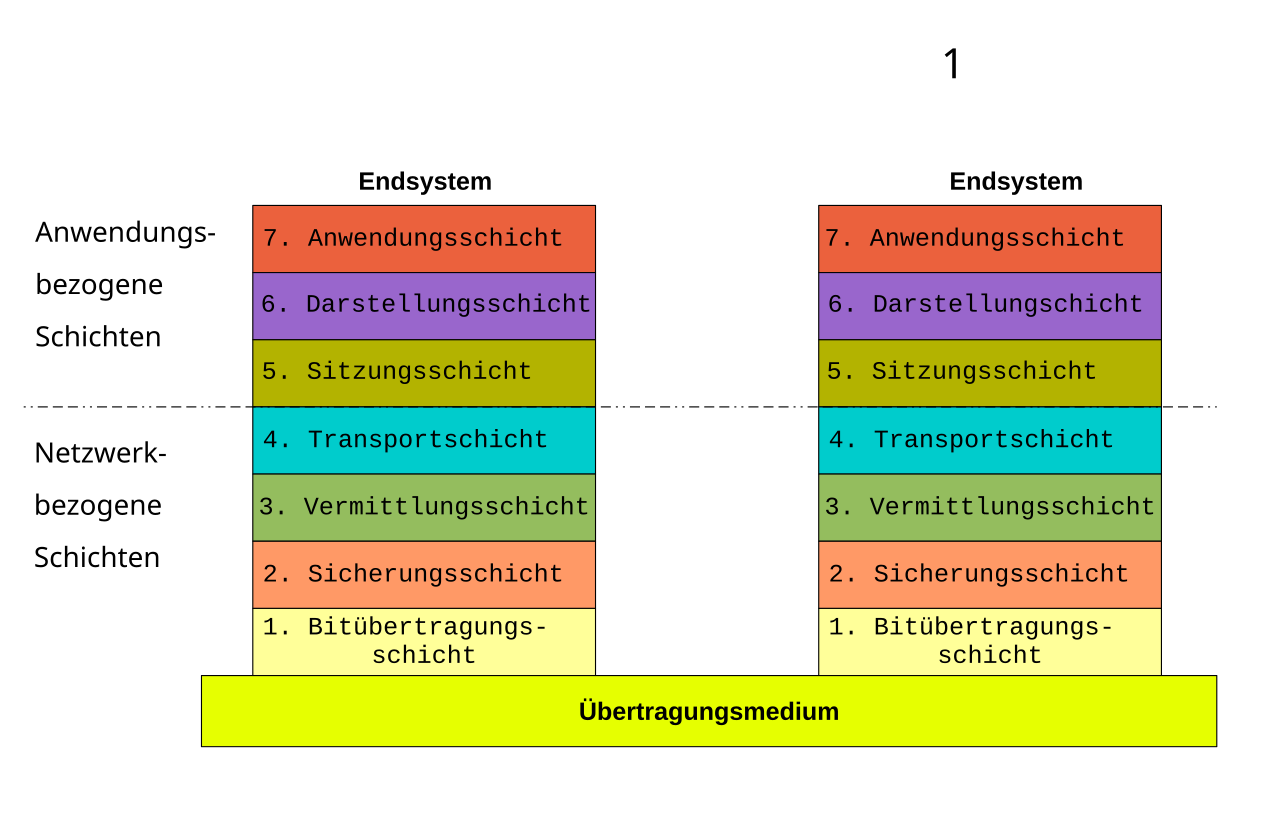
\includegraphics[width=0.75\linewidth]{picture-lib/osi.png}
    \caption{OSI Model Graphik von (Michael von Brandenburg)}
    \label{fig:placeholder}
\end{figure}

Die erste Schicht (\textbf{Die Bitübertragungsschicht}) ist die physische Schicht. Sie umfasst Antennen, Kabel, Hubs und ähnliche Hardware und dient als Medium, über das ein Bitstrom übertragen wird. Das geschieht über Kabel oder über elektromagnetische Wellen, wie beim WLAN.\\\\

Die zweite Schicht (\textbf{Die Sicherungsschicht}) regelt den Zugriff auf die physische Schicht. Sie sorgt für eine Datenflusskontrolle und dafür, dass alle Daten fehlerfrei übertragen werden. Sie besteht aus den zwei Unterschichten MAC (Media Access Control) und LLC (Logical Link Control). Die MAC-Adressen identifizieren die Hardware in einem Netzwerk. Typische Geräte dieser Schicht sind Bridges und Switches.\\\\

Die dritte Schicht (\textbf{Die Vermittlungsschicht}) vermittelt Datenpakete durch das ganze Netzwerk. Zu ihren Aufgaben gehören das Routing, also die Suche nach dem besten Weg zum Empfänger, und die Stauvermeidung bei hohem Netzwerkverkehr. Sie spielt vor allem bei Routern eine Rolle und versieht jedes Paket mit einer IP-Adresse, damit es beim richtigen Empfänger ankommt.\\\\

Die vierte Schicht (\textbf{Die Transportschicht}) sorgt dafür, dass die Datenpakete in der richtigen Reihenfolge beim Empfänger ankommen. Je nach Protokoll prüft sie auch, ob alle Pakete angekommen sind. Ausserdem weist sie den Paketen einen Port zu.\\\\

Die fünfte Schicht (\textbf{Die Sitzungsschicht}) baut eine Sitzung auf, behebt Probleme während der Sitzung und beendet sie wieder.\\\\

Die sechste Schicht (\textbf{Die Darstellungsschicht}) arbeitet wie ein Übersetzer zwischen den Daten der Anwendung und den Daten, die über das Netzwerk gehen. Sie kann Daten ausserdem komprimieren und verschlüsseln. Typische Beispiele sind UTF-8 für die Zeichenkodierung und AES für die Verschlüsselung.\\\\

Die siebte Schicht (\textbf{Die Anwendungsschicht}) verbindet den Benutzer mit den unteren Schichten. Beispiele sind Messaging-Apps und Browser. Sie nimmt die Daten des Benutzers entgegen und gibt sie an die unteren Schichten weiter.

\subsection{IP}

Das \textbf{IP} (Internet Protocol) ist eine der Grundlagen des Internets. Es gibt zwei Standards, den älteren IPv4 und den neueren IPv6, und sie unterscheiden sich im Adressraum. IPv4 erlaubt nur 2\textsuperscript{32} (4 294 967 296) Adressen, IPv6 dagegen 2\textsuperscript{128}. Das sind so viele, dass man nie erleben wird, dass sie aufgebraucht sind. Eine IP-Adresse kann man sich wie die Adresse eines Gebäudes vorstellen. Jedes Gebäude hat eine eindeutige Adresse, und genauso hat ein Router eine eindeutige öffentliche Adresse. IPv4 musste ersetzt werden, weil es nicht mehr genügend eindeutige Adressen gab. IPv6 bringt zudem Verbesserungen bei der Sicherheit.\\\\


Jedes Datenpaket, das über das Netzwerk verschickt wird, braucht eine Adresse, sonst findet es seinen Empfänger nicht. Ausserdem möchte man nicht der ganzen Welt mitteilen, was man gestern gefrühstückt hat.

\subsection{TCP}

Das \textbf{TCP} (Transmission Control Protocol) bildet zusammen mit dem IP das TCP/IP-Protokoll, das heute überall als Standard verwendet wird. Beim Netzwerk-Engineering benutzt man oft das OSI-Modell, in der Praxis läuft aber TCP/IP. Wie in Abbildung (...) zu sehen ist, findet man die meisten Elemente des OSI-Modells wieder, nur die fünfte und die sechste Schicht fehlen. Ihre Aufgaben übernimmt im TCP/IP-Modell die Anwendungsschicht. Trotzdem spricht man im Sprachgebrauch weiterhin von sieben Schichten. TCP ist ein zuverlässiges Protokoll der vierten Schicht und stellt sicher, dass alle Datenpakete richtig ankommen. Dafür verwendet es einen Three-Way-Handshake, eine Sequenzierung und eine Checksumme.

\subsection{UDP}

Das \textbf{UDP} (User Datagram Protocol) ist ebenfalls ein Protokoll der vierten Schicht. Es ist weniger zuverlässig als TCP, wird aber dort eingesetzt, wo ein schneller Datenaustausch wichtiger ist als ein kleiner Datenverlust, zum Beispiel beim DNS (Domain Name System) oder bei Anrufen.

\section{Multithreading}

\subsection{Thread}

Ein \textbf{Thread} (Ausführungsstrang) ist ein Programmablauf. Braucht ein Programm mehr als einen Thread, spricht man von Multithreading. Mit mehreren Threads lassen sich Aufgaben parallel berechnen, sodass nicht jede Funktion auf die vorherige warten muss. Als Beispiel kann man ein Programm nehmen, das Kunden bedient. Mit nur einem Thread kann es nur einen Kunden aufs Mal bedienen. Mit zwei oder mehr Threads können mehrere Kunden gleichzeitig bedient werden, ohne dass sie auf den Kunden vor ihnen warten müssen.

\subsection{Daemon Thread}

in \textbf{Daemon Thread} ist ein Thread, der im Hintergrund läuft. Das Programm wartet nicht darauf, dass er fertig wird, und er endet automatisch, sobald alle normalen Threads beendet sind. Der Begriff leitet sich von Hintergrunddiensten (Daemons) ab.

\section{Verschlüsselung}

\subsection{Allgemeine Bedeutung}

\textit{"Bei der Verschlüsselung wird lesbarer Klartext in unlesbaren Chiffretext umgewandelt, um sensible Informationen vor unbefugten Benutzern zu verbergen. Unternehmen nutzen regelmäßig Verschlüsselung im Bereich Datensicherheit, um sensible Daten vor unberechtigtem Zugriff und Data Breaches zu schützen."}\citep{ai-wikipedia}\todo{Ändere die Quelle IBM Verschlüsselung}\\
Die \textbf{Verschlüsselung} gibt es schon seit mehreren tausend Jahren. Aus dem Altertum sind viele verschlüsselte Nachrichten dokumentiert. Die Methoden haben sich stetig weiterentwickelt, bis zu den heutigen Verfahren, die auch ein herkömmlicher Computer ohne den Schlüssel nicht entziffern kann. Der Grund dafür ist, wie das Zitat zeigt, der Schutz privater Daten vor unbefugten Personen. Im Netzwerk sind viele sogenannte "Black Hat"-Hacker unterwegs, die Daten stehlen und für hohe Summen zurück- oder weiterverkaufen. Würde man Daten nicht jederzeit verschlüsseln, würde man ihnen diese auf dem Silbertablett servieren.

\subsection{XOR}

Das \textbf{XOR-Gatter} (Exklusiv-Oder-Gatter) ist eine Schaltung, die ein Signal nur weiterleitet, wenn die beiden Eingangssignale verschieden sind. Sind sie gleich, gibt sie kein Signal weiter.

\[Y=A\veebar B\]
Mit XOR kann man auch Bits verschlüsseln. Das Verfahren allein ist aber leicht zu brechen, weil sich wiederholende Muster im Schlüssel eine Schwachstelle sind. Trotzdem bauen viele Verschlüsselungsverfahren auf XOR auf. Ein Bit hat nur zwei Zustände, wahr (1) oder falsch (0), und um diese zu verknüpfen, braucht es eine Schaltung wie das XOR.

\subsection{Advanced Encryption Standard (AES)}

Der \textbf{Advanced Encryption Standard} ist ein symmetrischer Verschlüsselungsalgorithmus, der in vier Operationen arbeitet, die in mehreren Runden wiederholt werden. Er gilt als Verschlüsselungsstandard, weil es nach heutigem wissenschaftlichem Stand keine Methode gibt, die Verschlüsselung zu brechen, ausser man besitzt den Schlüssel oder es passiert ein Fehler im Prozess selbst. Der Grund liegt im Aufbau des Algorithmus, der mit einer 4x4-Matrix arbeitet. Jede Zelle dieser Matrix enthält 1 Byte (8 Bit), insgesamt sind es also 16 Bytes (128 Bit). Der Schlüssel kann bei AES 128, 192 oder 256 Bit lang sein.\\\\
Zuerst wird eine \textbf{Substitutionsbox} (S-Box) konstruiert, mit der in der ersten Operation jedes Byte ersetzt werden kann. Mathematisch wird sie wie folgt berechnet:\\\\
\(\mathbb{F}_{2^8}\) ist ein endlicher Körper. Mit der Funktion \(S(x)\) wird für jedes Byte eine inverse und eine affine Transformation berechnet.
\[S(x)=\bar{x}\oplus(\bar{x}\lll1)\oplus(\bar{x}\lll2)\oplus(\bar{x}\lll3)\oplus(\bar{x}\lll4)\oplus(63)\small{hex}\]
\(\bar{x}\) ist die multiplikative Inverse von \(x\) in \(\mathbb{F}_{2^8}\). \(b\lll n\) ist die Linksrotation der Bits um \(n\) Positionen. \(\oplus\) ist die XOR-Verknüpfung.\\\\
Als Nächstes nimmt der Algorithmus den Schlüssel und erzeugt daraus \(R +1\) Teilschlüssel, von denen jeder in einer Runde verwendet wird. Insgesamt werden \(b\cdot(R+1)\) Bit benötigt, wobei \(b\) die Blockgrösse ist.\\\\
Für \(i=N,\dots,b/32\cdot(R+1)-1:\)
\[W_i=\left\{ \begin{array}{@{}lcl@{}}
W_{i-N}\oplus S(W_{i-1}\lll8)\oplus C_{i/N-1} & \mbox{wenn} & i \equiv 0 \mbox{ (mod } N)\\ W_{i-N}\oplus S(W_{i-1}) & \mbox{wenn} & N>6 \mbox{ und } \equiv 4 \mbox{ (mod }N)\\
W_{i-N}\oplus W_{i-1} & \mbox{sonst}
\end{array}\right.\]
Diese Formel beschreibt die \textbf{Schlüsselexpansion}, bei der der ursprüngliche Schlüssel erweitert wird, ohne dass ein leicht erkennbares Muster entsteht. Der Schlüssel wird zuerst in die Wörter \(W_0,\dots,W_{N-1}\) aufgeteilt und dann mithilfe von \(W_i\) erweitert. \(S(x)\) ist die S-Box-Funktion und sorgt für die Durchmischung. Für \(C_j\) berechnet man \(2^j\) im Körper \(\mathbb{F}_{2^8}\) und setzt das Ergebnis in das höchste Byte der Konstante \(C_j\) ein. In der Graphik (\todo{graphik}) ist das besser zu erkennen.\\\\
Die berechneten Rundenschlüssel werden in der vierten Operation (AddRoundKey) zur Matrix addiert. Die erste Operation ist \textbf{SubBytes}, bei der jedes Byte der Matrix in \(S(x)\) eingesetzt wird.\\ Danach folgt \textbf{ShiftRows}, bei dem die Zeilen der Matrix verschoben werden. Die erste Zeile bleibt unverändert, die zweite wird um eine Position verschoben, die dritte um zwei und die vierte um drei.\\ Dann folgt \textbf{MixColumns}, das die Spalten vermischt. Um das Byte \(b_j\) zu berechnen, wird jedes \(a_j\) der alten Spalte mit den Konstanten 1, 2 oder 3 multipliziert.

\begin{align}
b_0 = (a_0\cdot2)\oplus(a_1\cdot3)\oplus(a_2\cdot1)\oplus(a_3\cdot1)\\
b_1 = (a_0\cdot1)\oplus(a_1\cdot2)\oplus(a_2\cdot3)\oplus(a_3\cdot1)\\
b_2 = (a_0\cdot1)\oplus(a_1\cdot1)\oplus(a_2\cdot2)\oplus(a_3\cdot3)\\
b_3 = (a_0\cdot3)\oplus(a_1\cdot1)\oplus(a_2\cdot1)\oplus(a_3\cdot2)\\
\end{align}

Matrix:
\[\begin{pmatrix}
b_0\\ b_1\\ b_2\\ b_3 \\ 
\end{pmatrix}=
\begin{pmatrix}
2 & 3 & 1 & 1\\ 
1 & 2 & 3 & 1\\ 
1 & 1 & 2 & 3\\  
3 & 1 & 1 & 2 
\end{pmatrix}\begin{pmatrix}
a_0\\ a_1\\ a_2\\ a_3 \\ 
\end{pmatrix}\]
Im Galois-Körper \(GF(2^8)\) gilt:

\begin{align}
&a\cdot1=a\\
&a\cdot2=\left\{ \begin{array}{@{}lcl@{}}
2a & \mbox{wenn} & a < 2^7\\
2a\oplus(11b)\small{hex} & \mbox{wenn} & a \geq 2^7\\
\end{array}\right.\\
&a\cdot3=(a\cdot2)\oplus a
\end{align}


Die letzte Operation ist AddRoundKey. Sie verknüpft den Rundenschlüssel per XOR mit der Matrix und beendet damit einen Durchgang der Schleife. Dieser wird je nach Schlüssellänge 10, 12 oder 14 Mal wiederholt: Je länger der Schlüssel, desto mehr Runden werden benötigt. Die Entschlüsselung läuft genau umgekehrt ab.

\section{Datenpakete}

\subsection{Aufbau}

Der Aufbau eines \textbf{Datenpakets} hängt vom Protokoll ab. Man könnte auch ein eigenes Protokoll verwenden, aber kein anderes Gerät könnte es lesen, weil überall das Standardprotokoll TCP/IP verwendet wird. Dieses folgt der OSI-Struktur ohne die Sitzungs- und die Darstellungsschicht. Das Datenpaket wird zuerst in der Anwendungsschicht aufgebaut. Als Beispiel nehme ich den Verbindungsaufbau zu einer Webseite. In der Anwendungsschicht wird HTTPS festgelegt, entweder weil der Benutzer den Link selbst eingegeben hat oder weil das DNS die richtige Seite gefunden hat. Das erste Stück besteht aus dem HTTPS-Teil und den Daten, die an die nächste Schicht weitergegeben werden. In der Transportschicht kommt ein L4-Header (Layer 4) dazu, der festlegt, ob TCP oder UDP verwendet wird, und der die Portnummer enthält. In der Vermittlungsschicht wird der L3-Header hinzugefügt, der die Source-IP und die Destination-IP enthält. In der Sicherungsschicht wird das Paket von einem L2-Header und einem L2-Trailer umhüllt und wird so zu einem Frame. Dieser enthält die MAC-Adressen von Sender und Empfänger. Zum Schluss wird das Paket über die Bitübertragungsschicht verschickt, bis es beim Zielgerät ankommt, in diesem Fall beim Server der Webseite.

\subsection{Translation}

Datenpakete enthalten alle diese Informationen als Bytes. Computer können sie leicht lesen, für Menschen sind sie aber unbrauchbar. Ausserdem sind Nachrichten meist verschlüsselt. Darum braucht es die Darstellungsschicht, die den Binärcode in Zeichen umwandelt. Das geschieht mit ASCII oder UTF-8, wobei jede Bitkombination einem Zeichen zugeordnet wird. Die Ver- und Entschlüsselung findet vor beziehungsweise nach dieser Übersetzung statt.